\documentclass[a4paper, 11pt]{article}

\setcounter{tocdepth}{3}
\setcounter{secnumdepth}{3}

\usepackage{comment} % enables the use of multi-line comments (\ifx \fi) 
\usepackage{lipsum} %This package just generates Lorem Ipsum filler text. 
\usepackage{fullpage} % changes the margin
\usepackage[utf8]{inputenc}
\usepackage{gensymb}
\usepackage{graphicx}
\usepackage{booktabs}% http://ctan.org/pkg/booktabs
\usepackage{makecell}
\usepackage{tabularx}
\usepackage[table]{xcolor}
\usepackage{array}
\usepackage{wrapfig}
\usepackage{subcaption}
\usepackage{csquotes}
\usepackage{lscape}
\usepackage{afterpage}
\usepackage{geometry}
\usepackage{listingsutf8}
\usepackage{chngcntr}
\usepackage{multicol}
\usepackage{xcolor}


\counterwithin{figure}{section}

\geometry{a4paper, margin=1in}
\renewcommand{\figurename}{Abb.}
\renewcommand{\tablename}{Tabelle}
\newcommand{\code}[1]{\texttt{#1}}

\renewcommand*{\thead}[1]{\bfseries #1}

\renewcommand{\contentsname}{Inhalt}
\renewcommand{\listfigurename}{Abbildungsverzeichnis}

\definecolor{lightgray}{rgb}{.9,.9,.9}
\definecolor{darkgray}{rgb}{.4,.4,.4}
\definecolor{purple}{rgb}{0.65, 0.12, 0.82}
\definecolor{darkgreen}{rgb}{0.05,0.56,0.06}

\lstdefinelanguage{JavaScript}{
	keywords={typeof, new, true, false, catch, function, return, null, catch, switch, var, if, in, while, do, else, case, break},
	keywordstyle=\color{blue}\bfseries,
	ndkeywords={class, export, boolean, throw, implements, import, this},
	ndkeywordstyle=\color{darkgray}\bfseries,
	identifierstyle=\color{black},
	sensitive=false,
	comment=[l]{//},
	morecomment=[s]{/*}{*/},
	commentstyle=\color{purple}\ttfamily,
	stringstyle=\color{darkgreen}\ttfamily,
	morestring=[b]',
	morestring=[b]"
}

\lstset{frame=tlrb,
	language=JavaScript,
	aboveskip=3mm,
	belowskip=3mm,
	showstringspaces=false,
	columns=flexible,
	basicstyle={\small\ttfamily},
	numbers=left,
	numberstyle=\tiny\color{gray},
	keywordstyle=\color{blue},
	commentstyle=\color{violet},
	stringstyle=\color{darkgreen},
	breaklines=true,
	breakatwhitespace=true,
	tabsize=3,
	literate=%
	{Ö}{{\"O}}1
	{Ä}{{\"A}}1
	{Ü}{{\"U}}1
	{ß}{{\ss}}1
	{ü}{{\"u}}1
	{ä}{{\"a}}1
	{ö}{{\"o}}1
}


\begin{document}
	
\title{Zusammenfassung WEBAPP FS2018}
\author{Alex Neher}
\maketitle

\tableofcontents
\newpage
\listoffigures
\newpage

\graphicspath{{./Pictures/}}

\section{JavaScript}
Javascript, auch ECMAScript genannt ist eine clientseitige web-Development Sprache für DOM- und CSS-Manipulation, AJAX oder EventHandling. Javascript kann in HTML-Code eingebunden werden, entweder inline über \code{<script></script>}-Tags, es kann mittels \code{<script src=path/to/file.js></script>} geholt werden oder direkt über EventHandler \code{<input type="checkbox" name="options" onchange="order.options.giftwrap = this.checked;">}. 

\subsection{Variablen definieren}

Javascript hat keine Typisierung. Das heisst, Variablen können einfach mit dem Keyword \code{var} definiert werden, ohne dass ein Datentyp spezifiziert werden muss.

\begin{lstlisting}
var a = 2;  // a ist nun eine Nummer
a = 'Jetzt bin ich ein String';
a = false;
\end{lstlisting}

\subsection{Funktionen}
In Javascript werden Funktionen als Objekte behandelt. Sie können ebenfalls mit dem Keyword \code{var} erstellt werden. Jede Funktion hat ihren eigenen Kontext/Scope. Jede Funktion hat per Default zwei Parameter: \code{this} und \code{arguments}.

Der \code{this} Parameter gibt den Kontext der Funktion zurück. Dieser hängt davon ab, wie und wo die Funktion aufgerufen wird. \code{arguments} ist ein Array, in welchem alle mitgegebenen Argumente speichert.

\begin{lstlisting}
//1. Über anonymes Function Literal
var add = function(a,b){
	console.log(arguments[0]) //gibt den Wert von a zurück
	return a+b;
}

//2. Über Function Literal mit Name
var sub = function sub(a,b){
	return a-b;
}

//3. Über Function Declaration
function mult(a,b){
	return a*b;
}

//4. Über Immediate Function Invocation
var TenDividedByTwo = function(a,b){return a/b;}(10,5);
console.log(TenDividedByTwo) //Output: 5
\end{lstlisting}

Funktionen können auch direkt in Objekten definiert werden
\begin{lstlisting}
var person = {
	firstName = "Thomas",
	lastName = "Koller",

	printFullName: function(){
		console.log(this.firstName + " " + this.lastName);
	};
}

person.printFullName();
\end{lstlisting}

Mit dem 'apply'-Pattern können auch Funktionen von anderen Objekten aufgerufen werden

\begin{lstlisting}
var anotherPerson = {
	firstName = "Donald",
	lastName = "Trump"
}

anotherPerson.printFullName() //error: undefined

aPerson.printFullName.apply(anotherPerson); //Output: Donald Trump
\end{lstlisting}

Wie bereits erwähnt, werden Funktionen als Objekte behandelt und haben ihren eigenen Kontext/Scope. Das heisst, von ausserhalb kann nicht direkt auf Variablen innerhalb einer Funktion zugegriffen werden, sondern nur über verschachtelte Funktionen. Dieses Konstrukt nennt man \textbf{Closure}.

\begin{lstlisting}
var myCounter = (function(){
	var value = 0;
	return {
		increment: function(inc){
			value =+ inc;
		},
		getValue: function(){
			return value;
		}
	};
}());

myCounter.increment(10) //value = 10
console.log(myCounter.value); //error: undefined
console.log(myCounter.getValue()); //10
\end{lstlisting}


\subsection{Objekte}
JavaScript kann auch objektbasiert programmiert werden. Es gibt grundsätzlich vier Möglichkeiten, Objekte zu instanziieren:

\begin{lstlisting}
//1. über "var"
var bachelorModule = {
	title: "Webapplication Development",
	instructor: "Thomas Koller"
};

//2. über new und dem default-Konstruktor
var bachelorModule = new Object();

//3. über Object.create()
var bachelorModule = Object.create(Object.prototype); //ein leeres Objekt

//4. mit einem bereits bestehenden Objekt als Prototyp
var masterModule = Object.create(bachelorModule) //ist jetzt ein "Klon" von bachelorModule
\end{lstlisting}

Der Zugriff auf Properties funktioniert wie bei anderen objektorientierten Sprachen

\begin{lstlisting}
console.log(bachelorModule.title);  //Output: Webapplication Development
console.log(bachelorModule["instructor"]); //Output: Thomas Koller
\end{lstlisting}

Objekte sind dynamisch. Das heisst, es können zur Laufzeit noch Properties hinzugefügt oder entfernt werden:

\begin{lstlisting}
//hinzufügen von Properties
bachelorModule.credits = 3;

//entfernen von Properties
delete bachelorModule.credits;

//Ebenfalls kann gecheckt werden, ob ein Property existiert
bachelorModule.hasOwnProperty("title"); //true
bachelorModule.hasOwnProperty("credits"); //false
\end{lstlisting}

JavaScript hat, wie auch andere objektorientierten Sprachen, Konstruktoren (die immer gross geschrieben werden)

\begin{lstlisting}
function Name(vorname, nachname){
	this.vorname = vorname;
	this.nachname = nachname;
	this.birthDate = {
		year: 0,
		month: 0,
		day: 0
	}
}
\end{lstlisting}

\paragraph{Prototyp}\mbox{}\\

Wie bereits im Kapitel 'Funktionen' beschrieben, können Funktionen direkt in Objekten definiert werden. Dann existieren sie jedoch nur für diese eine Objekt (z.B. dem Objekt aPerson). Wenn ich nun eine Funktion definieren will, die für alle \code{Name}-Objekte existiert, muss ich sie mithilfe dem \code{prototype}-Keyword definieren.

\begin{lstlisting}
Name.prototype.hello = function(){
	console.log("Hello " + this.vorname); 
}

var aPerson = new Name("Thomas", "Koller");
aPerson.hello();
\end{lstlisting}

Diese Methode funktioniert, da jedes Objekt ein Prototype hat. Wenn ein gesuchtes Property nicht im Objekt-eigenen Prototype gefunden, so wird rekursiv im Prototype des Prototype-Objekts gesucht, bis man ganz oben bei \code{Object} angekommen ist. Falls dort immer noch nichts gefunden wurde, wird \code{null} zurückgegeben. 

Wenn ein Objekt mithilfe der \code{Object.create()}-Methode instanziiert wird, so hat das neu erstellte Objekt den Prototypen des mitgegebenen Objekts.

\begin{lstlisting}
var obj1 = {
	a: 1
}

var obj2 = Object.create(obj1); //Der Prototyp von obj2 ist jetzt obj1

console.log(obj2.a) //Output: 1
\end{lstlisting}

\code{obj2} selbst hat kein 'a'-Property, es wird also eine Stufe höher gesucht, im Property von \code{obj2}, also \code{obj1}

\subsection{Arrays}

\begin{lstlisting}
//Instanziierung von Arrays über var
var emptyArray = [];
var numberArray = [1, 3, 6];

//Instanziierung von Arrays über new
var anotherEmptyArray = new Array();
var arrayOfFive = new Array(5);

//Da JavaScript keine Typisierung kennt, sind auch gemsiche Arrays möglich
var mixedArray = ["String", 4, true];

//Es können auch Objekte in Arrays verpackt werden
var modulesArray = [
	{title:"WEBAPP", instructor:"Koller"}, 
	{title:"WEBTEC", instructor:"Infanger"}
];

//Zugriff und hinzufügen von Array-Elemente erfolgt gleich wie bei bekannten Sprachen
console.log(numberArray[0]) //1
numberArray[3] = "new Element"

//Arrays müssen nicht zwingend ganz gefüllt sein
var sparseArray = new Array(1000);
console.log(sparseArray[500]); //undefined
\end{lstlisting}

\subsection{JavaScript und JSON}
Javascript erlaubt die direkte Konvertierung von Objekten zu JSON. Die Methode \code{JSON.stringify()} ruft die Methode \code{toJSON()} auf (falls diese existiert) und serialisiert das zurückgegebene Objekt.

Um JSON wieder in ein Objekt zurückzuverwandeln, ruft man \code{JSON.parse()} auf.

\begin{lstlisting}
var json = JSON.stringify(bachelorModule));
//Output: {"title":"WebApp","instructor":"Thomas Koller"}

var otherBachelorModule = JSON.parse(json);
\end{lstlisting}

\newpage

\subsection{Verarbeitung von JavaScript}
\begin{wrapfigure}[18]{R}{0.75\textwidth}
	\centering
	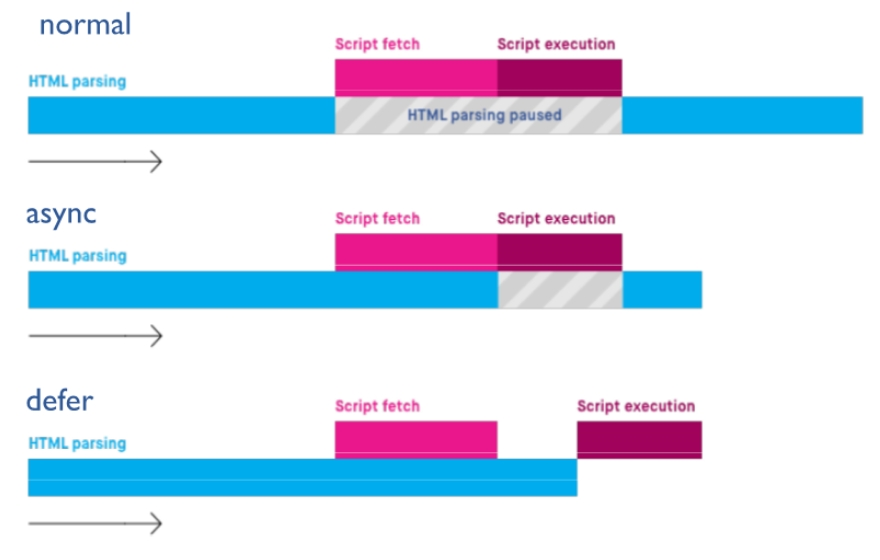
\includegraphics[keepaspectratio=true,height=15\baselineskip]{js_ausfuehrung.jpg}
	\caption{Verschiedene Arten, wie JS verarbeitet werden kann}
	\label{fig:rel}
\end{wrapfigure}
JavaScript kann normal, asynchron oder deferred ausgeführt werden. Bei der normalen Verarbeitung wird das HTML-Parsing pausiert, das JS-Skript heruntergeladen, kompiliert und ausgeführt und erst anschliessend mit dem HTML-Parsing weitergemacht. Wenn man die asynchrone Verarbeitung wählt, wird das JS-Skript im Hintergrund heruntergeladen. Erst wenn das Skript heruntergeladen wurde, wird das HTML-Parsing pausiert und das Skript wird ausgeführt. Bei der deferred-Methode wird das Skript ebenfalls im Hintergrund heruntergeladen. Jedoch wird hier gewartet, bis das gesamte HTML-Parsing abgeschlossen ist, bevor das Skript ausgeführt wird.

\subsection{Verzögerte Ausführung}

Mittels den Methoden \code{long setInterval(function f, unsigned long interval, any args)} und \code{long setTimeOut(function f, unsigned long timeout, any args)} kann die Ausführung der übergebenen Methode verzögert (setTimeOut) oder in einem definierten Intervall wiederholt (setInterval) werden. Die Ausführung der Methode \code{f} wird um \code{timeout} Millisekunden verzögert bzw. nach \code{interval} Millisekunden wiederholt.

\subsection{DOM}
\begin{figure}[htb]
	\centering
	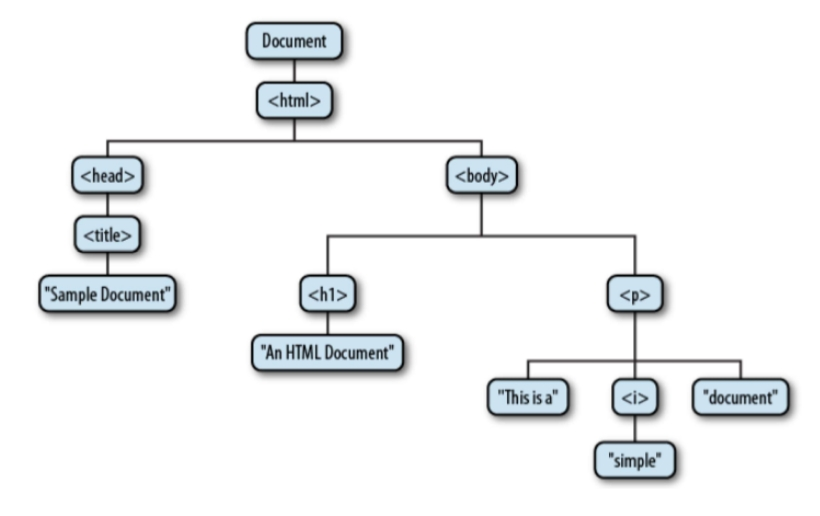
\includegraphics[keepaspectratio=true,height=14\baselineskip]{DOM_structure.jpg}
	\caption{Beispiel eines DOM-Baumes}
	\label{fig:DOM}
\end{figure}
DOM steht für \textit{Document Object Model} und bezeichnet die Struktur einer HTML-Website. Alle Objekte der Website werden in der Baumstruktur des DOMs als Node abgespeichert. JavaScript kann direkt auf diese Nodes zugreifen z.B. wäre \code{"simple"} in Abb. \ref{fig:DOM} mittels \code{document.childNodes[0].childNodes[1].lastChild.firstChild.nextSibling.childNodes[0]} erreichbar. Da dies jedoch ein bisschen umständlich ist, werden im nächsten Kapitel einige einfachere Selektions-Methoden vorgestellt.

\subsection{DOM-Manipulation}
Wie bereits zu Beginn des Kapitels erwähnt, wird JavaScript unter anderem zur DOM-Manipulation verwendet. Um Elemente des DOM manipulieren zu können, muss dem Skript zuerst mitgeteilt werden, welches Element man manipulieren möchte. Dabei gibt es verschiedene Methoden:

\paragraph{Über ID (empfohlen)}\mbox{}\\
\begin{lstlisting}
var button = document.getElementById("button1")
\end{lstlisting}

\begin{lstlisting}[language=html]
<button id="button1">Click me!</button>
\end{lstlisting}

\paragraph{Über Namen}\mbox{}\\
Diese Methode gibt eine NodeList zurück mit allen gefundenen Elementen
\begin{lstlisting}
var buttons = document.getElementsByName("option_buttons")
console.log(buttons[0].tagName) //Output: button
\end{lstlisting}
\begin{lstlisting}[language=html]
<button name="option_button">Pizza Margharita</button>
<checkbox name="option_button">Pizza Diavola</checkbox>
\end{lstlisting}

\paragraph{Über Tags}\mbox{}\\
Funktioniert gleich wie \code{getElementsByName} aber filtert nach HTML-Tags
\begin{lstlisting}
var buttons = document.getElementsByTagName("button")
console.log(buttons[0].name) //Output: option_button
\end{lstlisting}
\begin{lstlisting}[language=html]
<button name="option_button">Pizza Margharita</button>
\end{lstlisting}

\paragraph{Über Klasse(n)}\mbox{}\\
Gibt eine HTML-Collection zurück. Falls mehrere Klassen spezifiziert werden, muss das Element Mitglied \textit{aller} Klassen sein
\begin{lstlisting}
var buttons = document.getElementsByClassName("options")
console.log(buttons[0].name) //Output: option_button
\end{lstlisting}
\begin{lstlisting}[language=html]
<button class="options">Pizza Margharita</button>
\end{lstlisting}

\paragraph{Über CSS-Selektoren}\mbox{}\\
Nur kompatibel mit HTML5. Gibt eine NodeList zurück.
\begin{lstlisting}
var logs = document.querySelectorAll("#log>span)
\end{lstlisting}
\begin{lstlisting}[language=html]
<div id=span>
	<span>I'm selected</span>
</div>
\end{lstlisting}

\section{PHP}
PHP ist eine serverseitige Script-Sprache. Also im Gegensatz zu JavaScript, bei welcher alles auf dem Computer des Benutzers berechnet wird, wird bei PHP alles bereits auf dem Webserver berechnet und nur die Resultate an den Browser des Benutzers geschickt. 

Ein PHP-Request läuft folgendermassen ab:

\begin{enumerate}
	\item Der Client ruft eine PHP-Seite auf
	\item Der Webserver leitet den Request an den PHP-Interpreter weiter
	\item Der Interpreter verarbeitet die Seite und  schickt das Resultat zurück an den Server
	\item Der Server schickt das Resultat zurück an den Client.
\end{enumerate}

PHP und HTML können in einer Datei gemischt werden.

\begin{lstlisting}[language=php]
<html>
	<head>
		<title>PHP-Stuff</title>
	</head>
	<body>
		<?php echo "Hello World"; ?>
	</body>
</html>
\end{lstlisting}

Variablen in PHP beginnen immer mit einem \code{\$} und müssen nicht zwingend zuerst deklariert werden. Strings werden, wie gewohnt, entwerder mit Doppel- oder Einfachanführungszeichen geschrieben. Ebenfalls bereits bekannt aus anderen Sprachen ist das Abschliessen eines Statements mit dem ';'

\vspace{10px}

\noindent PHP kann ebenfalls objektorientiert programmiert werden und hat Java/.NET ähnliche Kontrollstrukturen wie Schlaufen oder Konditionen. Externe PHP-Dateien können mittels \code{import} oder \code{include} importiert werden.

\vspace{10px}

\noindent Falls eine Webapplikation eine SQL-Datenbank im Backend hat, wird meist über PHP darauf zugegriffen

\begin{lstlisting}[language=php]
include 'db_credentials.php'

//$host, $user, $pass und $db sind im File 'db_credentials.php' gespeichert
$mysqli = new mysqli($host, $user, $pass, $db);

//mittels '->' kann auf Methoden zugegriffen werden, hier also die Methode 'query' vom mysqli-Objekt
$result = $mysqli->query("SELECT * from personen");

\end{lstlisting}

Nebst plainText und HTML-Seiten kann PHP noch andere Content-Types zurücksenden, es muss jedoch als erstes im Header mittels \code{header("Content-Type: whatever");} spezifiziert werden (z.B. JSON)


\end{document}